\documentclass[a4paper,10pt]{report}

\usepackage[utf8]{inputenc}
\usepackage{xspace}
\usepackage{graphicx,graphics} 
\usepackage{color}
\usepackage{amsmath}
\usepackage{amsfonts}
\usepackage{amssymb}
\usepackage{amsthm}
\usepackage{algorithm}
\usepackage{algorithmic}
\usepackage{longtable}
\usepackage{complexity}
\usepackage{tkz-graph}
\usepackage{float}
\usepackage{setspace}
\renewcommand{\algorithmicrequire}{\textbf{Input:}}
\renewcommand{\algorithmicensure}{\textbf{Output:}}
  
\graphicspath{{figures/}}
\newcommand\rmatching{${\cal R}$-matching\xspace}
\newcommand\mdelay{$\cal M$-delay\xspace}
\newcommand\matchedgraph{{\bf matched graph}}

\newcommand{\reporttitle}{Contention management for Deterministic Networking}     % Titre
\newcommand{\reportauthor}{Maël \textsc{Guiraud }} % Auteur
\newcommand{\reportsubject}{Master Thesis} 
\newcommand{\HRule}{\rule{\linewidth}{0.5mm}}
\setlength{\parskip}{1ex} % Espace entre les paragraphes


\newcommand{\todo}[1]{{\color{red} TODO: {#1}}}
\begin{document}


%Notice that the notion of $P$-periodic affectation \textbf{is not monotone} with regard to $P$. 
%Indeed, consider messages of size 1, we can build a ${\cal R}$-matching of a graph, with ${\cal L}$ routes $r_1, \dots, r_{{\cal L}-1}$ which all intersect two by two and such that if $r_i$ and $r_j$ have $v$ as first common vertex we have $\lambda(v,r_i) - \lambda(v,r_j)=1$.
%Therefore there is a $2$-periodic affectation by setting all $m_i$ to $0$.

A {\bf conflict graph} represents the collision between the routes of a routed network $N$. The vertices of a conflict graph $G = (V,E)$ are the routes of $N$, and there is an edge between two vertices if and only if there is a common arc between the two routes in the matched graph.
 
 Given $u$ and $v$ two vertices of the conflict graph, corresponding to two routes colliding in the matched graph. The weight of an edge, $w(u,v)$, is the absolute value of the difference between the distance of the two routes between their respective source node and the collision point.
 
 A labeling $F$ of such a graph is an affectation of an integer to each vertex, such that for each vertex $u$, $f(u) \neq f(v)+w(u,v)\mod P$, where $v$ are the neighbors of $u$ in the conflict graph and $P$ our period.
 
\begin{tabular}{cc}
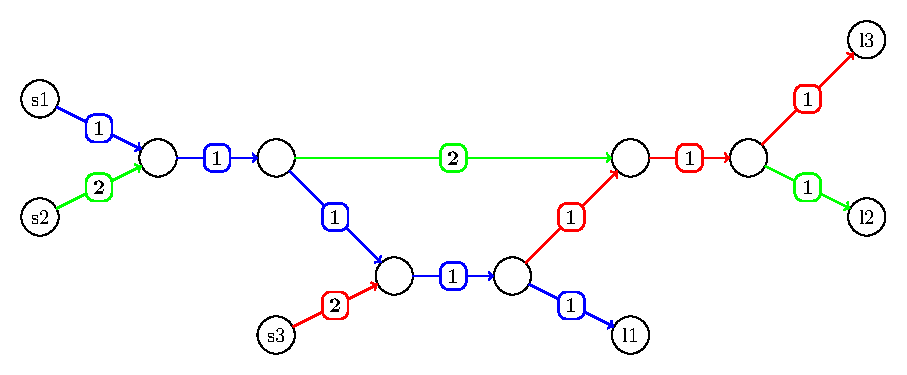
\includegraphics[scale=0.5]{Fig5.pdf} & 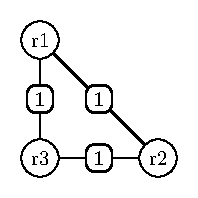
\includegraphics[scale=1]{Fig7.pdf}\\
 $\lambda(v,r_i) - \lambda(v,r_j)=1$ & Conflict graph\\
\end{tabular}\newline

\end{document}
